\documentclass[
  bibliography=totoc,     % Literatur im Inhaltsverzeichnis
  captions=tableheading,  % Tabellenüberschriften
  titlepage=firstiscover, % Titelseite ist Deckblatt
]{scrartcl}

% Paket float verbessern
\usepackage{scrhack}

% Warnung, falls nochmal kompiliert werden muss
\usepackage[aux]{rerunfilecheck}

% unverzichtbare Mathe-Befehle
\usepackage{amsmath}
% viele Mathe-Symbole
\usepackage{amssymb}
% Erweiterungen für amsmath
\usepackage{mathtools}

% Ableitungen
\usepackage{esdiff}

% Fonteinstellungen
\usepackage{fontspec}
% Latin Modern Fonts werden automatisch geladen
% Alternativ zum Beispiel:
%\setromanfont{Libertinus Serif}
%\setsansfont{Libertinus Sans}
%\setmonofont{Libertinus Mono}

% Wenn man andere Schriftarten gesetzt hat,
% sollte man das Seiten-Layout neu berechnen lassen
\recalctypearea{}

% deutsche Spracheinstellungen
\usepackage[ngerman]{babel}
\usepackage{textalpha}


\usepackage[
  math-style=ISO,    % ┐
  bold-style=ISO,    % │
  sans-style=italic, % │ ISO-Standard folgen
  nabla=upright,     % │
  partial=upright,   % ┘
  warnings-off={           % ┐
    mathtools-colon,       % │ unnötige Warnungen ausschalten
    mathtools-overbracket, % │
  },                       % ┘
]{unicode-math}

% traditionelle Fonts für Mathematik
\setmathfont{Latin Modern Math}
% Alternativ zum Beispiel:
%\setmathfont{Libertinus Math}

\setmathfont{XITS Math}[range={scr, bfscr}]
\setmathfont{XITS Math}[range={cal, bfcal}, StylisticSet=1]

% Zahlen und Einheiten
\usepackage[
  locale=DE,                   % deutsche Einstellungen
  separate-uncertainty=true,   % immer Unsicherheit mit \pm
  per-mode=symbol-or-fraction, % / in inline math, fraction in display math
]{siunitx}

% chemische Formeln
\usepackage[
  version=4,
  math-greek=default, % ┐ mit unicode-math zusammenarbeiten
  text-greek=default, % ┘
]{mhchem}

% richtige Anführungszeichen
\usepackage[autostyle]{csquotes}

% schöne Brüche im Text
\usepackage{xfrac}

% Standardplatzierung für Floats einstellen
\usepackage{float}
\floatplacement{figure}{htbp}
\floatplacement{table}{htbp}

% Floats innerhalb einer Section halten
\usepackage[
  section, % Floats innerhalb der Section halten
  below,   % unterhalb der Section aber auf der selben Seite ist ok
]{placeins}

% Seite drehen für breite Tabellen: landscape Umgebung
\usepackage{pdflscape}

% Captions schöner machen.
\usepackage[
  labelfont=bf,        % Tabelle x: Abbildung y: ist jetzt fett
  font=small,          % Schrift etwas kleiner als Dokument
  width=0.9\textwidth, % maximale Breite einer Caption schmaler
]{caption}
% subfigure, subtable, subref
\usepackage{subcaption}

% Grafiken können eingebunden werden
\usepackage{graphicx}

% schöne Tabellen
\usepackage{booktabs}

% Verbesserungen am Schriftbild
\usepackage{microtype}

% Literaturverzeichnis
\usepackage[
  backend=biber,
]{biblatex}
% Quellendatenbank
\addbibresource{lit.bib}
\addbibresource{programme.bib}

% Hyperlinks im Dokument
\usepackage[
  german,
  unicode,        % Unicode in PDF-Attributen erlauben
  pdfusetitle,    % Titel, Autoren und Datum als PDF-Attribute
  pdfcreator={},  % ┐ PDF-Attribute säubern
  pdfproducer={}, % ┘
]{hyperref}
% erweiterte Bookmarks im PDF
\usepackage{bookmark}

% Trennung von Wörtern mit Strichen
\usepackage[shortcuts]{extdash}

% Aufrechtes d mit weniger Aufwand
\newcommand{\dif}{\mathrm{d}}

\setlength\parindent{0pt}

\author{%
  Jonas Ollesch\\%
  \href{mailto:jonas.ollesch@tu-dortmund.de}{jonas.ollesch@tu-dortmund.de}%
  \and%
  Lukas Annuss\\%
  \href{mailto:lukas.annuss@tu-dortmund.de}{lukas.annuss@tu-dortmund.de}%
}
\publishers{TU Dortmund – Fakultät Physik}


\subject{V46}
\title{Der Faraday Effekt}
\date{%
  Excution: 01.11.2023
  \hspace{3em}
  Hand-In: TT.MM.2023
}

\begin{document}

\maketitle
%\thispagestyle{empty}
%\tableofcontents
%\newpage
\setcounter{page}{1}

\section{Ziel des Versuches}
\label{sec:versuchsziel}
Ziel des Versuches ist es, die magnetische Flussdichte einer langen Spule und eines Helmholtzspulenpaares sowie die Hysteresekurve samt Remanenz und Koerzitivkraft einer Ringspule zu ermitteln.  
\section{Theoretische Grundlagen}
\label{sec:theorie}

\subsection{Entstehung und Zerfall kosmischer Myonen}

Treffen Protonen kosmischer Höhenstrahlung auf die Moleküle der Luft, entstehen unter anderem Pionen und Kaonen, die daraufhin einen hadronischen Teilchenschauer auslösen können. \\
Die hier betrachteten kosmischen Myonen sind ein Teil dieses Luftschauers, der direkt aus den Pion- und Kaonzerfällen entsteht. \\

Unter Erzeugung eines Myons und Myonneutrinos zerfallen diese wie folgt:

\begin{align*}
    \pi^- &\rightarrow \mu^- + \bar{\nu}_\mu \\
    \pi^+ &\rightarrow \mu^+ + \nu_\mu \\
    K^+ &\rightarrow \mu^+ + \nu_\mu \,.
\end{align*}

Die in etwa $10 - 15 \,\unit{\kilo\meter}$ \cite{grup} entstehenden Myonen besitzen die selben Eigenschaften wie Elektronen, mit dem Unterschied, dass Myonen etwa die 200-fache Masse \cite{pdg} besitzen .
Auch mit einer Lebensdauer von etwa $2,187 \cdot 10^{-6} \,\unit{\second}$ \cite{pdg} erreicht aufgrund der hochrelativistischen Geschwindigkeiten etwa 
$1 \,\text{Myon} \, (\unit{\centi\meter}^2 \, \unit{\minute})^{-1}$ die Erdoberfläche \cite{grup}. \\

Erreicht ein Myon das Ende seiner Lebensdauer, zerfällt es unter Austausch eines W-Bosons über den folgenden Kanal:

\begin{equation*}
    \mu \rightarrow e + \nu_e + \nu_\mu \,,
\end{equation*}

wobei immer ein Neutrino und ein Antineutrino so entsteht, dass die Leptonzahl erhalten bleibt. \\
Für positive Myonen ist dieser Zerfall der einzig mögliche, negative Myonen können dagegen auch durch Myoneinfang zerfallen.
Dabei wird das wie ein Elektron negativ geladene Myon von einem Atomkern angezogen und löst aufgrund seiner gegenüber Elektronen größeren Masse eine Elektronenkaskade aus,
bis es auf das niedrigste Energieniveau fällt und vom Kern unter Entstehung eines Neutrons und eines Neutrinos eingefangen wird:

\begin{equation*}
    \mu^- + p \rightarrow n + \nu_\mu \,.
\end{equation*}

Dadurch erhält das negative Myon genau genommen eine geringere Lebensdauer.


\subsection{Berechnung der Lebensdauer}

Zur Berechnung der Lebensdauer wird im Folgenden von einem exponentiellen Zusammenhang der Form
\begin{equation}
    N(t) = N_0 \, e^{-\lambda \, t}
    \label{eq:expdec}
\end{equation}
zwischen der Anzahl der Myonen zum Zeitpunkt $t_0 = 0$ und der Zeit $t$ ausgegangen. 
Dabei bezeichnet $N_0$ die Anzahl der Myonen zu Beginn, $N(t)$ die Anzahl nach einer Zeit $t$ und $\lambda$ die charakteristische Zerfallskonstante des Prozesses. \\

Die Lebensdauer $\tau$ lässt sich mit dem zeitlichen Erwartungswert $<t>$ identifizieren.
Es gilt
\begin{equation}
    \tau = <t> = \int_0^\infty \text{d} t \, \lambda \, t \, e^{-\lambda \, t} = \frac{1}{\lambda} \,.
\end{equation} 

Für diesen Versuch muss \eqref{eq:expdec} um einen Untergrund $B$ ergänzt werden, um alle gezählten Ereignisse zu beschreiben, sodass
\begin{equation}
    N(t) = N_0 \, e^{-\lambda \, t} + B
\end{equation}
gilt.

Zur Abschätzung dieses Hintergrundes treffe innerhalb einer Suchzeit $T_\text{s}$ nach Eintreffen des ersten Myons ein weiteres als unerwünschter Untergrund ein.
Für die durchschnittliche Anzahl gemessener Myonen pro Sekunde während der gesamten Messzeit $T_\text{mess}$ gilt
\begin{equation*}
    n = \frac{N_\text{start}}{T_\text{mess}} \,,
\end{equation*}
wobei $N_\text{start}$ die Anzahl der gegebenen Startsignale, also die Anzahl der eintreffenden "ersten" Myonen beschreibt. \\

Das Produkt $T_\text{s} \cdot n$ beschreibt den Erwartungswert der Messungen in der Suchzeit. \\

Damit lässt die poissonverteilte Wahrscheinlichkeit für das Eintreffen $k$ weiterer Myonen durch
\begin{equation*}
    P(k) = \frac{(T_\text{s} \cdot n)^k}{k!} \, e^{T_\text{s} \cdot n}
\end{equation*}
beschreiben. \\

Über
\begin{equation*}
    N_\text{fehl} (k) = N_\text{start} \cdot P(k)
\end{equation*}
lässt sich so die Anzahl der Fehlereignisse berechnen, wobei hier insbesondere $N(1)$ wichtig ist.

\newpage

\subsection{Erklärung wichtiger Bauelemente}

Die Erklärung der im Versuch verwendeten Bauelemente erfolgt nach \autoref{fig:schaltung}.

\begin{figure}
    \centering
    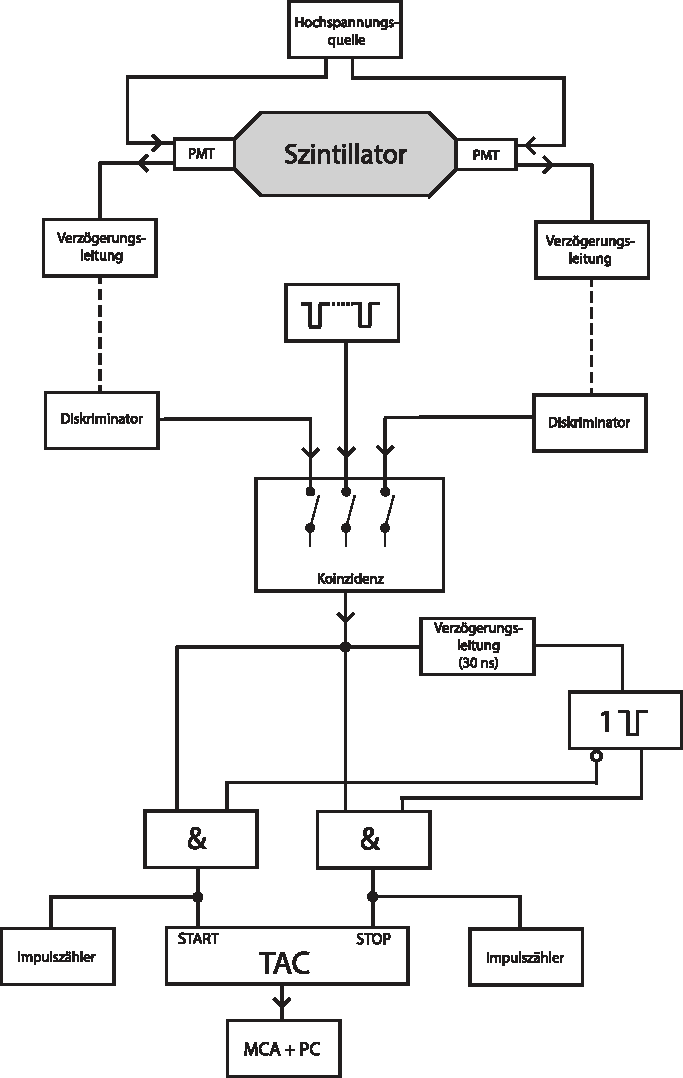
\includegraphics[width=.6\textwidth]{figures/V01.pdf}
    \caption{Schaltbild der verwendeten Messelektronik \cite{ap03}.}
    \label{fig:schaltung}
\end{figure}

\subsubsection{Szintillator}

Bei dem ersten verwendeten Bauteil handelt es sich um einen flüssigen organischen Szintillator. Der Unterschied zu anorganischen Szintillatoren besteht darin, dass hier nicht das Szintillatormaterial
ionisiert wird und sich ein Elektron zum Aktivierungszentrum bewegen muss, um ein Photon auszulösen, sondern dass das Szintillatormaterial auf ein höheres Energieniveau angeregt wird.
Diese Anregungsenergie wird innerhalb einiger Nanosekunden wieder freigesetzt \cite{kolawerm}. \\
Die Zeitauflösung organischer Szintillatoren ist deutlich höher als die anorganischer Szintillatoren.
Aufgrund der Vielfalt unterschiedlicher Anregungsniveaus organischer Szintillatoren ist die Energieauflösung verglichen mit den diskreten Ionisationsenergien der anorganischen Szintillatoren geringer.
Für Lebensdauermessung ist besonders die Zeitauflösung wichtig, also eignen sich organische Szintillatoren am besten. \\


\subsubsection{Photomultiplier}

Der Photomultiplier (PMT) wandelt mithilfe des Photoeffekts ein eintreffendes Photon in ein elektrisches Signal um.
Über eine anliegende Beschleunigungsspannung wird das vom Photon ausgelöste Elektron zur Anode beschleunigt und löst auf seinem Weg weitere Elektronen aus.
An der Anode lassen sich diese Elektronen als Strom messen.
Insgesamt wird das vom Szintillator eintreffende Signal um einen Faktor von bis zu $10^9$, für gewöhnlich um $10^5 - 10^7$-fach, verstärkt \cite{kolawerm}.


\subsubsection{Verzögerungsleitung}

In den Verzögerungsleitungen liegen Leitungen unterschiedlicher Länge, sodass das eintreffende Signal mit Schaltern über die Leitungen umgeleitet werden kann.
Das Signal legt eine längere Strecke zurück und ist damit verzögert. Die hier verwendeten Verzögerungsleitungen verfügen über sieben unterschiedliche Schalter, mit denen Einzelverzögerung
zwischen $1 \,\unit{\nano\second}$ und $32 \,\unit{\nano\second}$ eingestellt werden können. Diese Schalter funktionieren additiv.


\subsubsection{Diskriminator}

Die verbauten Diskriminatoren verfügen über eine regelbare Schwellamplitude. Alle eintreffende Impulse unter dieser Amplitude werden nicht weitergegeben, sodass unerwünschte Störsignale,
die beispielsweise durch zufällig ausgelöste Elektronen im PMT entstehen, unterdrückt.


\subsubsection{Koinzidenz}

Die Koinzidenz liefert nur dann einen Output, wenn an allen Eingängen gleichzeitig ein Eingangssignal eintrifft.


\subsubsection{Monostabile Kippstufe}

Die monostabile Kippstufe, auch Monoflop genannt, besitzt zwei unterschiedliche Zustände. Trifft ein Impuls am Monoflop ein, wird dieser von seinem Grundzustand in den angeregten Zustand geschaltet,
in dem er für eine definierbare Zeit verbleibt, bevor er sich wieder umschaltet. Dabei gibt er in beiden Positionen ein Signal aus.


\subsubsection{Time-Amplitude-Converter}

Der Time-Amplitude-Converter (TAC) verfügt über zwei Eingänge. Treffen zwei Signale nicht gleichzeitig ein, gibt er ein Ausgangssignal, dessen Amplitude proportional zum zeitlichen Abstand der beiden
Eingangssignale ist.


\subsubsection{Vielkanalanalysator}

Der Vielkanalanalysator (engl. Multichannel Analyser (kurz MCA)) sortiert Eingangssignale nach ihrer Amplitude in unterschiedliche Kanäle, erstellt also ein Histogramm der Eingangsdaten.






\section{Durchführung}
\label{sec:Durchführung}

Es wird durch ein schwenkbares Photoelement die Intensität eines Laser, der von einer Si-Oberfläche reflektierten Strahlung gemessen \autoref{fig:aufbau}.
Zwischen dem Laser und der Si-Oberfläche wird zusätzlich ein Polfilter platziert, damit das senkrecht vom parallel polarisierten Licht getrennt werden kann.
Die Si-Oberfläche ist auf einer Drehscheibe montiert, damit der Einfallswinkel des Laserlichts variiert werden kann. Das Photoelement muss immer so ausgerichtet werden, dass das Licht direkt in die Öffung des Photoelements fällt.
Ein Amperemeter misst den Strom, welcher durch den Laser im Photoelement erzeugt wird. Der gemessene Strom ist proportional zur Intensität, also zum Quadrat der Feldstärke.
Zunächst wird der Nullstrom gemessen, also die direkte Leistung des Lasers.

\begin{figure}[H]
    \centering
    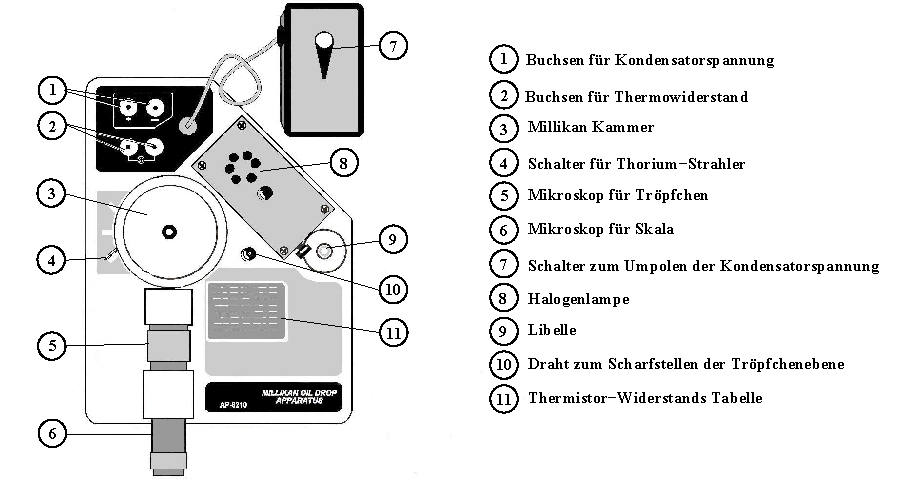
\includegraphics{Aufbau.pdf}
    \caption{Schematische Darstellung der Messapperatur \cite{ap01}.}
    \label{fig:aufbau}
\end{figure}

\section{Auswertung}
\label{sec:Auswertung}

\subsection{Bestimmung der Winkelrichtgröße}
\label{subsec:a}
Mithilfe von \eqref{eq:drehmombetrag} lässt sich \eqref{eq:winkelrichtgröße} zu
\begin{equation}
  D = \frac{F r}{\varphi}
  \label{eq:WinkelrichtgröFr}
\end{equation}
umschreiben. 

Die bei der ersten Messung aufgenommenen Daten sind in \autoref{tab:Messung_a} dargestellt.
Dabei ist $\varphi$ die Auslenkung des Systems und $F$ die am im Abstand von $r = 0,2 \,\unit{\meter}$ Kraftmesser gemessene rücktreibende Kraft. 
\begin{table}[H] % Hier noch eine dritte Spalte mit den einzelnen Winkelrichtgrößen wär nicht schlecht...
  \centering
  \sisetup{table-format=3.0}
  \begin{tabular}{S S[table-format=1.3]}
      \toprule
      {$\varphi\mathbin{/}\unit{°}$} & {$F \mathbin{/} \unit{\newton}$}\\
      \midrule
           30  & 0,042 \\
           40  & 0,062 \\
           50  & 0,088 \\
           60  & 0,106 \\  
           70  & 0,128 \\
           80  & 0,140 \\
           90  & 0,168 \\
           100 & 0,190 \\
           110 & 0,200 \\
           120 & 0,250 \\
      \bottomrule
  \end{tabular}
  \caption{Rücktreibende Kraft zu verschiedenen Auslenkungen.}
  \label{tab:Messung_a}
\end{table}

%Mittelwert und Standardabweichung hinschreiben
Aus den gemessenen Werten wurde der Mittelwert und die Standardabweichung berechnet.
Für die Winkelrichtgröße ergibt sich dann  
\begin{equation*}
  D = (0,0203 \pm 0,0020) \,\unit{\newton\meter} \,.  
\end{equation*}

\subsection{Bestimmung des Eigenträgheitsmoments}
\label{subsec:b}
% Was ist mit den Unsicherheiten auf den Messwerten, zumindest auf dem Gewicht? Hatten wir die? Ja wir hatten da eine, aber Katja hat in ihrem Protokoll auch keine angegeben xD
Um das Eigenträgheitsmoment zu bestimmen, wurden zwei Zylinder mit einer Masse von je $222,7 \,\unit{g}$, einem Radius von $16 \,\unit{mm}$ und einer Höhe von $27,1 \,\unit{mm}$ senkrecht zur Drehachse befestigt.
Der Abstand $a$ wurde dabei stets bis zum vorderen Ende des Zylinders gemessen und $\dfrac{h}{2}$ addiert, in \autoref{tab:Messung_b} 
sind also die Abstände bis zum Zylinderzentrum mit den dazugehörigen Schwingungsdauern dargestellt.

\begin{table}[H] % Hier statt 3T lieber 1T auftragen?? Ich meine, Katja hatte das schon beim ersten Protokoll erwähnt, dass 3T unnötig ist...
  %dann gibts halt nur T xD
  \centering
  \begin{tabular}{S[table-format=2.3] S[table-format=2.2]}
      \toprule
      {$a \mathbin{/}\unit{cm}$} & {$T \mathbin{/} \unit{\second}$}\\
      \midrule
           20,355 & 6,166 \\
           21,355 & 6,542 \\
           22,355 & 6,576 \\
           23,355 & 6,856 \\  
           24,355 & 7,109 \\
           25,355 & 7,329 \\
           26,355 & 7,646 \\
           27,355 & 7,793 \\
           28,355 & 8,113 \\
           29,355 & 8,406 \\
      \bottomrule
  \end{tabular}
  \caption{Schwingungsdauern $T$ bei verschiedenen Abständen $a$.}
  \label{tab:Messung_b}
\end{table}
Für das Trägheitsmoment wird die Form $ I = T_D + 2I_z + 2m a^2$ angenommen. 
Durch einsetzen in \eqref{eq:periodendauer} ergibt sich \eqref{eq:periodendauerquadrat}, dabei ist $I_z$ das Trägheitsmoment eines Zylinders, $m$ die Masse und $a$ der Abstand zur Rotationsachse.
\begin{equation}
  T^2 = 4 \pi^2 \frac{I_D}{D} + 8 \pi^2 \frac{m (\frac{R^2}{4} + \frac{h^2}{12})}{D}+ 8 \pi^2 \frac{m}{D} a^2 .
  \label{eq:periodendauerquadrat}
\end{equation}
In \autoref{fig:T2ga2} wird nun das Quadrat der Schwingungsdauer $T^2$ gegen das Abstandquadrat $a^2$ aufgetragen.
Die dazu durchgeführte lineare Regression nimmt die Form $T^2 = A  a^2 + B $ mit den Parametern
\begin{equation*}
  A = (708 \pm 20) \dfrac{1}{s^2m^2}
\end{equation*}
\begin{equation*}
 B = (8,8 \pm 1,3) \dfrac{1}{s^2} 
\end{equation*}
an.

Mithilfe von \eqref{eq:trägüschwi} lässt sich das Eigenträgheitsmoment zu
\begin{equation*}
  I_D = (0,0045 \pm 0,0008) \,\unit{\newton\meter} \,.
\end{equation*}
bestimmen.

Die Unsicherheit berechnet sich dabei aus der Gaußschen Fehlerfortpflanzung mit
\begin{equation}
  Δf(x_1,...,x_N) = \sqrt{\sum_{i=1}^N \left(\frac{\partial f}{\partial x_i}Δx_i\right)^2}
  \label{eq:gaußfehler}
\end{equation}
berechnen.

\begin{figure}[H]
  \centering
  \includegraphics{build/T2ga2.pdf}
  \caption{Lineare Regression der quadrierten Messwerte.}
  \label{fig:T2ga2}
\end{figure}

\subsection{Trägheitsmoment der Kugel}
\label{subsec:c}

Ähnlich zu \autoref{subsec:b} wird nun die Schwingungsdauer einer Kugel mit Durchmesser $d = 12,75 \, \unit{\centi\meter}$ und einer Masse von $m = 811,3 \,\unit{\gram}$ bestimmt und in \autoref{tab:Messung_c} dargestellt.
Die Messung wird mit einer Auslenkung von $\varphi = \dfrac{π}{2} = 90 \,\unit{\degree}$ zehn Mal wiederholt, die Schwingungsdauern werden gemittelt und es wird die Abweichung bestimmt.

\begin{table}[H] % Auch hier lieber noch 1T :D ✓ 
  \centering
  \begin{tabular}{S[table-format=2.0] S[table-format=1.2]}
      \toprule
      {Messung} & {$T \mathbin{/} \unit{\second}$}\\
      \midrule
          1  & 1,626 \\
          2  & 1,586 \\
          3  & 1,686 \\
          4  & 1,576 \\  
          5  & 1,626 \\
          6  & 1,559 \\
          7  & 1,663 \\
          8  & 1,753 \\
          9  & 1,646 \\
          10 & 1,626 \\
      \bottomrule
  \end{tabular}
  \caption{Schwingungsdauern $T$ der Kugel.}
  \label{tab:Messung_c}
\end{table}
Es ergibt sich die Periodendauer
\begin{equation*}
  T= (1,64 \pm 0,05) \, \unit{\second} \,.
\end{equation*}

Aus \eqref{eq:trägüschwi} ergibt sich das Trägheitsmoment der Kugel zu
\begin{equation*}
  I_{K,m} = (0,00138 \pm 0,00017)\, \unit{\newton\meter}  \, .
\end{equation*} \\

Wie in \autoref{fig:trägmomSKZ} zu sehen, ergibt sich der Theoriewert des Trägheitsmoments einer Kugel aus
\begin{equation}
  I_{K} = \frac{2}{5} m R^2
  \label{trägheitsmomK}
\end{equation}
zu
\begin{equation*}
  I_{K,t} = 0,00131 \, \unit{\newton\meter}. % die theorischen Werten haben keine Unsicherheit aber wenn die noch eine bekommen sollen, dann kann man da bestimmt noch was machen xD
\end{equation*}

Die relative Abweichung des gemessenen und theoretischen Wertes beträgt dann
\begin{equation*}
  \left|\frac{I_{K,m}}{I_{K,t}} * 100 - 100 \right| = 5,344 \% \,.
\end{equation*}



\subsection{Trägheitsmoment des Zylinders}
\label{subsec:d}

Analog zur Bestimmung des Trägheitsmoments der Kugel wird nun für den Zylinder vorgegangen. Mit einer Masse von $367,7 \,\unit{\gram}$, einer Höhe von $h = 9,74 \,\unit{\centi\meter}$
und einem Durchmesser von $d = 9,67 \,\unit{\centi\meter}$ ergeben sich für zehn Messungen die in \autoref{tab:Messung_d} dargestellten Schwingungsdauern.

\begin{table}[H]
  \centering
  \begin{tabular}{S[table-format=2.0] S[table-format=1.2]}
      \toprule
      {Messung} & {$T \mathbin{/} \unit{\second}$}\\
      \midrule
          1  & 0,90 \\
          2  & 0,77 \\
          3  & 0,86 \\
          4  & 0,82 \\  
          5  & 0,75 \\
          6  & 0,77 \\
          7  & 0,88 \\
          8  & 0,77 \\
          9  & 0,79 \\
          10 & 0,81 \\
      \bottomrule
  \end{tabular}
  \caption{Schwingungsdauern $T$ des Zylinders.}
  \label{tab:Messung_d}
\end{table}

Gemittelt ergibt sich hier die Schwingungsdauer
\begin{equation*}
  T = (0,82 \pm 0,05) \, \unit{\second} \,.
\end{equation*}

Das experimentelle Trägheitsmoment lässt sich erneut aus \eqref{eq:trägüschwi} zu
\begin{equation*}
  I_{K,m} = (0,00034 \pm 0,00004) \, \unit{\newton\meter}
\end{equation*} 
bestimmen. \\

Mit dem Trägheitsmoment
\begin{equation}
  I_Z = \frac{1}{2} m R^2
\end{equation}
eines aufrecht zur Drehachse stehenden Zylinders ergibt sich für den Theoriewert
\begin{equation*}
  I_{Z,t} = 0.00043 \,  \unit{\newton\meter}.
\end{equation*}

Die Abweichung beträgt dann
\begin{equation*}
  \left|\frac{I_{Z,m}}{I_{Z,t}} * 100 - 100 \right| = 20,930 \% \,.
\end{equation*}

\newpage

\subsection{Trägheitsmoment einer Holzpuppe}
\label{subsec:e}

Abschließend soll das Trägheitsmoment einer Holzpuppe in zwei unterschiedlichen Positionen bestimmt werden. Dazu wurden zunächst die einzelnen Körperteile abgemessen.
Für die Längen $l$ ergaben sich die in \autoref{tab:Messung_e1} aufgetragenen Werte, die je zehnfach gemessenen Durchmesser $d$ der einzelnen Körperteile finden sich in \autoref{tab:Messung_e2}.
Dabei sei eine Unsicherheit von $1 \, \unit{\milli\meter}$ anzunehmen.

\begin{table}[H]
  \centering
  \begin{tabular}{S[table-format=2.0] S[table-format=2.2]}
      \toprule
      {Körperteil} & {$l \mathbin{/} \unit{\meter}$}\\
      \midrule
        {Kopf}  & {$0.04310 \pm 0.00010$} \\
        {Arme}  & {$0.12920 \pm 0.00010$} \\
        {Torso} & {$0.08740 \pm 0.00010$} \\
        {Beine} & {$0.14630 \pm 0.00010$} \\
      \bottomrule
  \end{tabular}
  \caption{Längen der einzelnen Puppenkörperteile.}
  \label{tab:Messung_e1}
\end{table}

\begin{table}[H]
  \centering
  \sisetup{table-format=1.2}
  \begin{tabular}{S[table-format=2.0] S S S S}
      \toprule
      {Messung} & {$d_{Kopf} \mathbin{/} \unit{\centi\meter}$} & {$d_{Arme} \mathbin{/} \unit{\centi\meter}$} & {$d_{Torso} \mathbin{/} \unit{\centi\meter}$} & {$d_{Beine} \mathbin{/} \unit{\centi\meter}$} \\
      \midrule
        1  & 3.02 & 1.24 & 3.22 & 1.25 \\
        2  & 2.96 & 1.57 & 3.55 & 1.47 \\
        3  & 2.53 & 1.26 & 3.17 & 1.14 \\
        4  & 1.58 & 1.40 & 2.84 & 1.86 \\  
        5  & 2.92 & 1.10 & 2.59 & 1.31 \\
        6  & 2.48 & 0.96 & 2.74 & 1.17 \\
        7  & 2.02 & 1.32 & 2.50 & 1.03 \\
        8  & 2.87 & 1.30 & 3.27 & 0.99 \\
        9  & 2.03 & 0.85 & 3.35 & 1.01 \\
        10 & 1.59 & 1.22 & 3.46 & 1.22 \\
      \bottomrule
  \end{tabular}
  \caption{Durchmesser der einzelnen Puppernkörperteile.}
  \label{tab:Messung_e2}
\end{table}

Nach Mittelung der gemessenen Durchmesser ergeben sich die in \autoref{tab:Messung_e3} dargestellten Radien.

\begin{table}[H]
  \centering
  \begin{tabular}{S[table-format=2.0] S[table-format=2.2]}
      \toprule
      {Körperteil} & {$\bar{d} \mathbin{/} \unit{\meter}$}\\
      \midrule
        {Kopf}  & {$0,0120 \pm 0,0050$} \\
        {Arme}  & {$0,0061 \pm 0,0020$} \\
        {Torso} & {$0,0153 \pm 0,0035$} \\
        {Beine} & {$0,0062 \pm 0,0025$} \\
      \bottomrule
  \end{tabular}
  \caption{Gemittelte Radien der einzelnen Puppenkörperteile.}
  \label{tab:Messung_e3}
\end{table}

\subsubsection{Bestimmung des Trägheitsmoments in Position 1}
\label{subsubsec:pos1}

Zunächst soll das Trägheitsmoment der Holzpuppe mit seitlich ausgestreckten Armen bestimmt werden.
Erneut werden dazu zehnfach die Schwingungsdauern gemessen, diesmal jedoch sowohl für eine Auslenkung von $\varphi = 90 \unit{\degree}$ als auch $\varphi = 120 \unit{\degree}$,
die Messwerte sind in \autoref{tab:Messung_f} aufgetragen.

\begin{table}[H]
  \centering
  \begin{tabular}{S[table-format=2.0] S[table-format=1.3] S}
      \toprule
      {Messung} & {$T \mathbin{/} \unit{\second}$ bei $\varphi = 90 \unit{\degree}$} & {$T \mathbin{/} \unit{\second}$ bei $\varphi = 120 \unit{\degree}$}\\
      \midrule
      1 & 0.663 & 0.660 \\
      2 & 0.533 & 0.663 \\
      3 & 0.663 & 0.663 \\
      4 & 0.623 & 0.663 \\
      5 & 0.553 & 0.643 \\
      6 & 0.597 & 0.753 \\
      7 & 0.600 & 0.643 \\
      8 & 0.597 & 0.667 \\
      9 & 0.597 & 0.643 \\
      10& 0.710 & 0.597 \\
      \bottomrule
  \end{tabular}
  \caption{Schwingungsdauern bei Auslenkungen von $\varphi = 90 \unit{\degree}$ und $\varphi = 120 \unit{\degree}$ \\ in Position 1.}
  \label{tab:Messung_f}
\end{table}

Wie schon bei der Trägheitsmomentsbestimmung der anderen Körper kann nun erneut \eqref{eq:trägüschwi} genutzt werden, um das Trägheitsmoment zu berechnen.
Aus den gemittelten Schwingungsdauern ergeben sich dann
\begin{equation*}
  I_{P_1,1} = (0.00019 \pm 0.00004) \, \unit{\newton\meter} 
\end{equation*} 
für $\varphi = 90 \, \unit{{\degree}}$ und

\begin{equation*}
  I_{P_1,2} = (0.000224 \pm 0.000034) \, \unit{\newton\meter} 
\end{equation*}
für $\varphi = 120 \unit{\degree}$, erneut gemittelt also

\begin{equation*}
  I_{P_1,m} = (0.00022 \pm 0.00003) \, \unit{\newton\meter} \,.
\end{equation*}

Für die Berechnung des theoretischen Trägheitsmoments werden die einzelnen Körperteile als Zylinder approximiert. Dabei sei angenommen, dass die Drehachse genau durch den Mittelpunkt von Kopf und Torso verläuft, es gilt also
\begin{equation*}
  I_{Kopf,t} = \frac{1}{2} \, m_{Kopf} \, R^2_{Kopf}
\end{equation*}
und
\begin{equation*}
  I_{Torso,t} = \frac{1}{2} \, m_{Torso} \, R^2_{Torso} \,.
\end{equation*}

Dabei sind die Beine vertikal um je $R_{Beine}$ und die Arme horizontal um $\frac{h_{Arme}}{2} + R_{Torso}$ zur Drehachse verschoben. 
Über den Satz von Steiner lassen sich jetzt die dazugehörigen Trägheitsmomente berechnen.
Es ergeben sich mithilfe der Zylinderträgheitsmomente aus \autoref{fig:trägmomSKZ}
\begin{equation*}
  I_{Arme,t} = I_{Arme,S} + m a^2 = m \left(\frac{R^2_{Arme}}{4} + \frac{h^2_{Arme}}{12} \right) + m \left(R_{Torso} + \frac{h_{Arme}}{2} \right)^2
\end{equation*}
und
\begin{equation*}
  I_{Beine,t} = I_{Beine,S} + m a^2 = \frac{1}{2} \, m_{Beine} \, R^2_{Beine} + m \, R^2_{Beine}\,.
\end{equation*}

Das Gesamtträgheitsmoment setzt sich dann aus der Summe der Einzelträgheitsmomente zu
\begin{equation*}
  I_{P_1,t} = (0.00028 \pm 0.00015) \, \unit{\newton\meter}
\end{equation*}
zusammen.

\newpage

\subsubsection{Bestimmung des Trägheitsmoments in Position 2}
\label{subsubsec:pos2}

Analog wird nun für die zweite Puppenposition verfahren. 
Nun sind die Arm horizontal nach hinten und die Beine horizontal nach vorne ausgerichtet. 
In \autoref{tab:Messung_g} sind erneut die Schwingungsdauern dargestellt.

\begin{table}[H]
  \centering
  \begin{tabular}{S[table-format=2.0] S[table-format=1.3] S}
      \toprule
      {Messung} & {$T \mathbin{/} \unit{\second}$ bei $\varphi = 90 \unit{\degree}$} & {$T \mathbin{/} \unit{\second}$ bei $\varphi = 120 \unit{\degree}$}\\
      \midrule
      1  & 0.903 & 0.833 \\
      2  & 0.947 & 0.990 \\
      3  & 0.993 & 0.907 \\
      4  & 0.947 & 0.880 \\
      5  & 0.903 & 0.863 \\
      6  & 1.013 & 0.950 \\
      7  & 1.013 & 1.013 \\
      8  & 0.883 & 0.970 \\
      9  & 0.947 & 0.993 \\
      10 & 0.883 & 0.970 \\
      \bottomrule
  \end{tabular}
  \caption{Schwingungsdauern bei Auslenkungen von $\varphi = 90 \, \unit{\degree}$ und $\varphi = 120 \, \unit{\degree}$ \\ in Position 2.}
  \label{tab:Messung_g}
\end{table}

Aus den gemittelten Schwingungsdauern lassen sich wie schon in \autoref{subsubsec:pos1} die gemessenen Trägheitsmomente bestimmen und zu
\begin{equation*}
  I_{P_2,m} = 0.00045 \pm 0.00006 \, \unit{\newton\meter}
\end{equation*}
mitteln.

Zur Berechnung des Theoriewertes wird analog vorgegangen, es ändert sich lediglich das Trägheitsmoment der Beine, die nicht länger vertikal, sondern horizontal ausgerichtet sind.
Mit 
\begin{equation*}
  I_{Beine,t} = I_{Beine,S} + m a^2 = m \left(\frac{R^2_{Beine}}{4} + \frac{h^2_{Beine}}{12} \right) + m \left(\frac{h_{Beine}}{2} \right)^2
\end{equation*}
ergibt sich aus der Summe der Einzelträgheitsmomente
\begin{equation*}
  I_{P_2,t} = (0.00066 \pm 0.00023) \, \unit{\newton\meter} \,.
\end{equation*} \\

\subsection{Abweichungen von Theorie und Messung}

Die Abweichungen von Theorie und Messung belaufen sich auf

\begin{equation*}
  100 * \left(\frac{I_{P_1,m}}{I_{P_1,t}} - 1\right) = 21,429 \%
\end{equation*}
und
\begin{equation*}
  100 * \left(\frac{I_{P_2,m}}{I_{P_2,t}} - 1\right) = 31,818 \% \,.
\end{equation*}

Zum Vergleich der experimentellen und theoretischen Werte werden im Folgenden insbesondere die Verhältnisse der Trägheitsmomente $\frac{I_{P_1}}{I_{P_2}}$ der einzelnen Positionen betrachtet.
Es ergibt sich mit
\begin{equation*}
  d_{m}= \frac{I_{P_1,m}}{I_{P_2,m}} = 0,489
\end{equation*}
und
\begin{equation*}
  d_{t} = \frac{I_{P_1,t}}{I_{P_2,t}} = 0,424 
\end{equation*}
die relative Abweichung von
\begin{equation*}
  d_{ges} = 100*(\frac{d_m}{d_t}-1) = 15,252 \,\% \,.
\end{equation*}
\section{Diskussion}

Als ausschlaggebende Fehlerquelle ist hier die fehlende Messung der Schwebegeschwindigkeit $v_0$ anzugeben.\\
Ohne diese Messreihe ist es nicht möglich, anhand von $v_\text{ab} - v_\text{auf} = 2 v_0$ eine Auswahl tatsächlich brauchbarer Werte zu treffen, sodass hier alle aufgenommenen Werte zur Auswertung verwendet wurden,
auch die der Tröpfchen, dessen Ladung sich unter Umständen im Laufe der Messung änderte. \\
Auch die nur begrenzte menschliche Reaktionszeit führt zu relativ groben Ungenauigkeiten und es ist zweifelhaft, dass die Methode, die den kleinsten gemeinsamen Nenner der Ladungen finden sollte, dies
tatsächlich getan hat.
Hier ergeben für die Elementarladung bei einem Literaturwert von $1,602176 \cdot 10^{-19} \,\si{\coulomb}$ \cite{elchar} und einem
Messwert von $\qty{5.2(0.8)e-19} \,\si{\coulomb}$ eine Abweichung von etwa $230 \,\%$, für die Avogadrokonstante sich bei einem Theoriewert von $6.02214076 \cdot 10^{23} \dfrac{1}{\si{\mol}}$ \cite{na} und einem Messwert von $\qty{1.85(0.29)e23} \,\dfrac{1}{\si{\mol}}$ eine Abweichung von knapp
$69 \,\%$. \\

Im Rahmen der groben Ungenauigkeiten der Messung ist es überraschend, dass die Elementarladung dennoch in derselben Größenordnung liegt. \\
Die Abweichung der Avogadrokonstante ist demnach relativ annehmbar.


\printbibliography{}
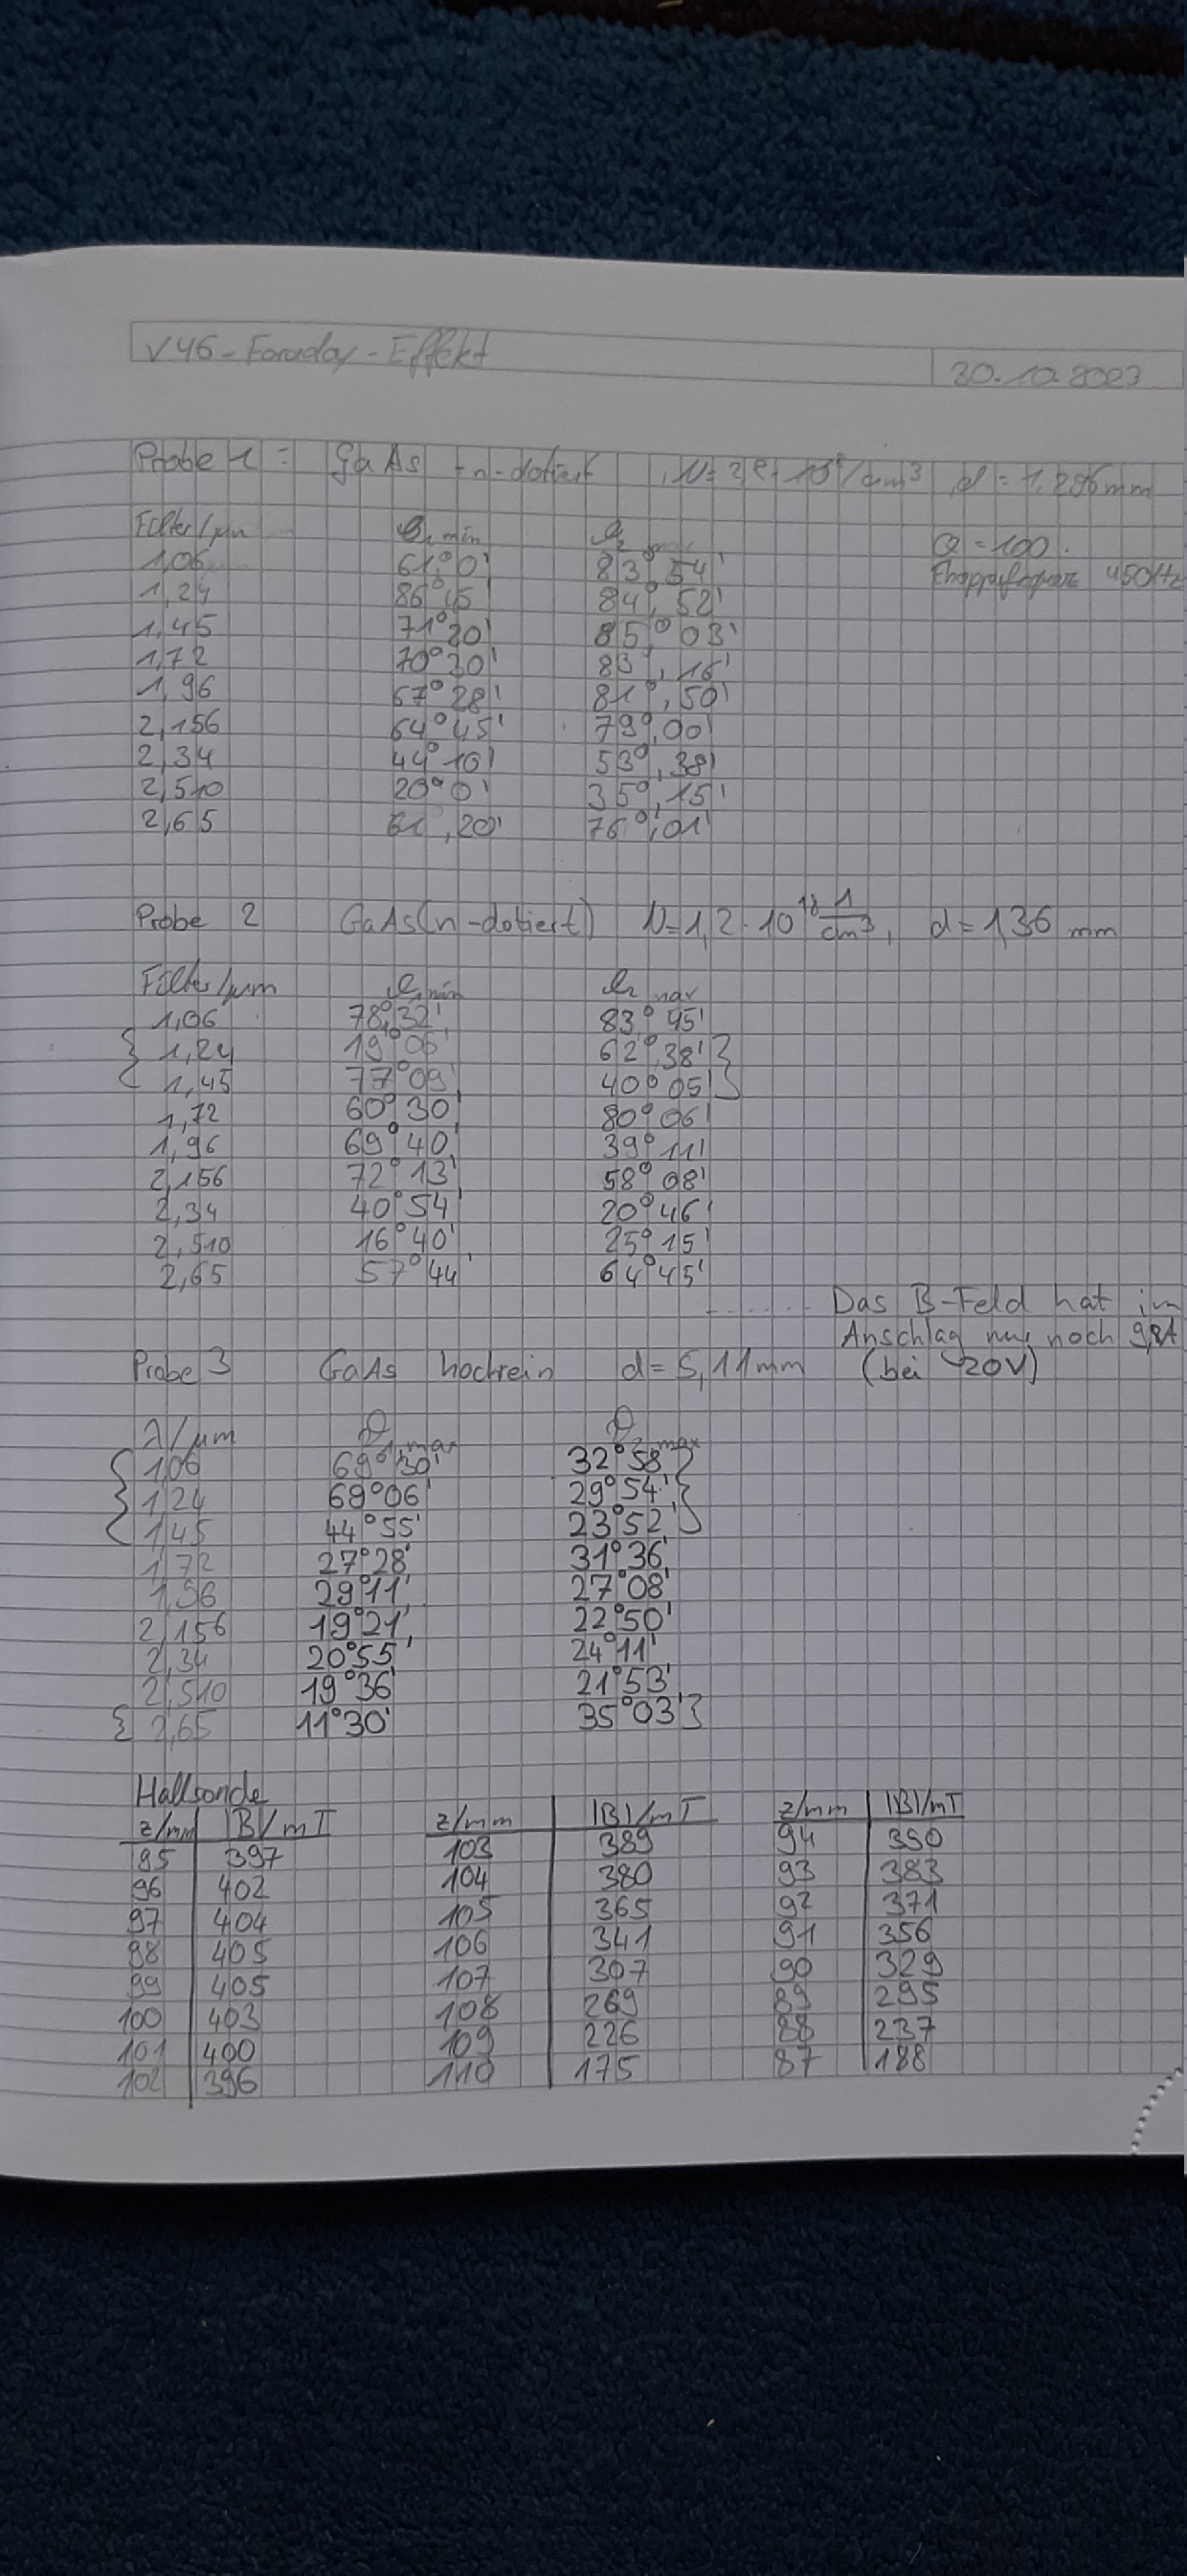
\includepdf[scale=0.75]{Messdaten/Messdaten.pdf}
\end{document}
